%%%%%%%%%%%%%%%%%%%%%%%%%%%%%%%%%%%%%%%%%
% Template LaTeX Template Version 1.0 (December 8 2014)
%
% This template has been downloaded from: http://www.LaTeXTemplates.com
%
% Original author: Brandon Fryslie With extensive modifications by: Vel
% (vel@latextemplates.com)
%
% License: CC BY-NC-SA 3.0 (http://creativecommons.org/licenses/by-nc-sa/3.0/)
%
% Authors: Sabbir Ahmed
% 
%%%%%%%%%%%%%%%%%%%%%%%%%%%%%%%%%%%%%%%%%

\documentclass[paper=usletter, fontsize=12pt]{article}
%%%%%%%%%%%%%%%%%%%%%%%%%%%%%%%%%%%%%%%%%
% Contract Structural Definitions File Version 1.0 (December 8 2014)
%
% Created by: Vel (vel@latextemplates.com)
% 
% This file has been downloaded from: http://www.LaTeXTemplates.com
%
% License: CC BY-NC-SA 3.0 (http://creativecommons.org/licenses/by-nc-sa/3.0/)
%
%%%%%%%%%%%%%%%%%%%%%%%%%%%%%%%%%%%%%%%%%

\usepackage{geometry} % Required to modify the page layout
\usepackage{multicol}
\usepackage{amsmath}
\usepackage{amssymb}

\usepackage[pdftex]{graphicx}
\usepackage{wrapfig}
\usepackage[font=scriptsize, labelfont=bf]{caption}
\usepackage[utf8]{inputenc} % Required for including letters with accents
\usepackage[T1]{fontenc} % Use 8-bit encoding that has 256 glyphs

\usepackage{avant} % Use the Avantgarde font for headings
\usepackage{courier}
\usepackage{xparse}
\usepackage{xcolor}
\usepackage{listings}  % for code verbatim and console outputs

\setlength{\textwidth}{16cm} % Width of the text on the page
\setlength{\textheight}{23cm} % Height of the text on the page
\setlength{\oddsidemargin}{0cm} % Width of the margin - negative to move text left, positive to move it right
\setlength{\topmargin}{-1.25cm} % Reduce the top margin

\setlength{\parindent}{0mm} % Don't indent paragraphs
\setlength{\parskip}{2.5mm} % Whitespace between paragraphs
\renewcommand{\baselinestretch}{1.5}

\definecolor{green}{rgb}{0.18, 0.55, 0.34}

\graphicspath{ {figures/} }
\captionsetup[table]{skip=10pt}

\lstset{language=C, keywordstyle={\bfseries \color{black}}}

% defines algorithm counter for chapter-level
\newcounter{nalg}[section]

%defines appearance of the algorithm counter
\renewcommand{\thenalg}{\thesection .\arabic{nalg}}

% defines a new caption label as Algorithm x.y
\DeclareCaptionLabelFormat{algocaption}{Algorithm \thenalg}

% defines the algorithm listing environment
\lstnewenvironment{pseudocode}[1][] {
    \refstepcounter{nalg}  % increments algorithm number
    \captionsetup{font=normalsize, labelformat=algocaption, labelsep=colon}
    \lstset{
        breaklines=true,
        mathescape=true,
        numbers=left,
        numberstyle=\scriptsize,
        basicstyle=\footnotesize\ttfamily,
        keywordstyle=\color{black}\bfseries,
        keywords={input, output, return, parallel, function, for, to, in, if,
        else, foreach, while, and, or, new, print},
        xleftmargin=.04\textwidth,
        #1
    }
}{}

\renewcommand{\familydefault}{\sfdefault}  % default font for entire document
 % specifies the document layout and style

\begin{document}

    \documentinfo {\textbf{Homework 6: Report}}
    {\today} {Sabbir Ahmed}
    \vspace{-0.1in}

    \section{Background} In this project students will learn to use generated
    IP Cores: a block RAM and a CORDIC processor for calculating square root.
    An essential skill to develop is the coding of a control finite state
    machine (FSM) to interface modules.

        \subsection{Requirements}

        \begin{itemize}

        \item The design should access 4 bytes from the serial port to initiate
        action

        \item The implementation should assume 4 bytes will be sent: ADDRESS-
        HIGH, ADDRESS-LOW, DATA-HIGH, DATA-LOW

        \item After 4 bytes are received the design should

        \begin{itemize}

            \item Read the contents of the RAM and send the HIGH-BYTE, then
            LOW-BYTE back through the UART

            \item Send the data bytes through the CORDIC Sqrt processor to
            compute the result

            \item The \texttt{sqrt} result just computed should be stored in
            the RAM at the same address that was just read

        \end{itemize}

        \item The hardware design should use 115200 baud rate and require NO
        modification to compile

        \item The design must include a simulation of the top-level design and
        discuss it in the report with a parameter to control baud rate. It is
        strongly recommended to consider modify the baud rate for the purpose
        of top-level simulation -- this should be controlled by a SINGLE
        parameter set in the test- bench. The design should not modify the UART
        implementation files.

        \item The FSM controller must as much as possible rely on use of status
        and control signals to manage the datapath timing, the design should
        not rely on "fixed" waits. This represents a better abstraction.

        \end{itemize}

    \section{Design Approach} The source code for interfacing with UART was
    provided. The controller FSM was implemented in 7 states visualized in
    Figure \ref{fig:states}. The module provides all the glue logic required to
    interface the UART with the \texttt{sqrt} module and the block RAM.

    \begin{figure}[ht]
        \begin{center}
            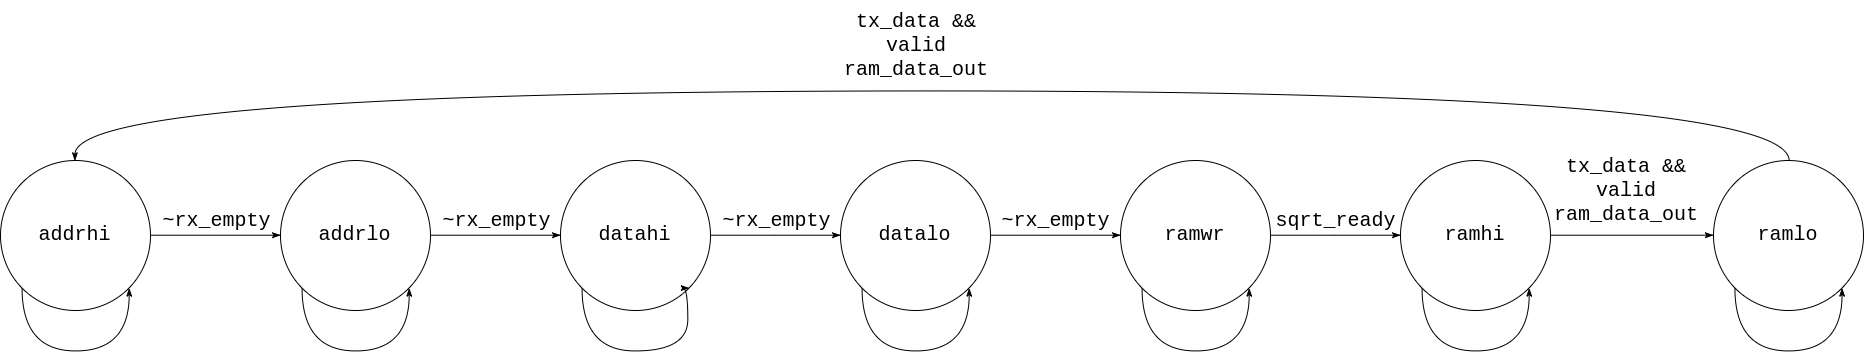
\includegraphics[width=1\textwidth]{state_diagram.png}
            \caption{State Diagram of the Implementation of the Controller}
            \label{fig:states}
        \end{center}
    \end{figure}

\end{document}
